\chapter{Ejercicio teleoperador acústico y banda sonora}\label{audio}
En los siguientes capítulos se explican los ejercicios desarrollados en este trabajo fin de grado. El primero de ellos es el teleoperador acústico. En este capítulo se nombran las herramientas utilizadas y como se ha realizado este ejercicio. También se muestra como se ha añadido la posibilidad de incluir efectos de sonido y bandas sonoras a los ejercicios ya existentes. 

\section{Teleoperador Acústico}
\subsection{Enunciado}
En este ejercicio se va a desarrollar un Teleoperador Acústico, el objetivo es crear un algoritmo de reconocimiento de voz con JavaScript para que un robot de Kibotics pueda ser dirigido con la voz. 

El alumno deberá indicarle  al robot con su voz órdenes claras para que el robot reconozca la orden en cada momento  y pueda moverse por el escenario sin chocar con ningún objeto. Hay dos escenarios disponibles, un muro de piedra y una portería de rugby, el dron deberá moverse por el mundo sin chocarse con ellos.

\subsection{Desarrollo del ejercicio}

Para empezar con este ejercicio utilizó un fichero de configuración sencillo en el que solo aparece un drone y un plano con una textura de césped. Este fichero de configuración es necesario para que el simulador Websim construya la escena 3D. El fichero de configuración esta escrito en JSON y Websim lo analiza para construir los mundos con A-Frame. 
Este sería una parte del fichero de configuración dende se muestra la configuración de la escena \textit{scene}, los robots\textit{robots\_config}, las texturas\textit{assets}y los objetos\textit{•objects}.

\begin{lstlisting}
{
    "scene-parent-id": "myIFrame",
    "scene": {
        "id": "scene",
        "gravity": 0,
        "sky": "../../assets/textures/sky.png",
        "background": "color: gray;",
        "inspector": "url: https://aframe.io/releases/0.4.0/aframe-inspector.min.js",
        "embedded": true,
        "physics": "debug: true"
    },
    "robots_config": [
        {
            "controller": "user1",
            "id": "a-pibot"
        }
    ],
    "assets": [
        {
            "tag": "img",
            "attr": {
                "id": "ground",
                "alt": "Texture for the scene ground",
                "src": "../../assets/textures/escenarioLiso-min.png"
            }
       ],
    "objects":[
     
        {
            "tag": "a-plane",
            "attr": {
                "static-body": {
                    "mass": 100000
                },
                "position": { "x":0, "y":0, "z":0 },
                "rotation": { "x":-90, "y":0, "z":0 },
                "width": "100",
                "height": "100",
                "src":"#ground"
            }
        },
        {
            "tag": "a-robot",
            "attr": {
                "id": "a-pibot",
                "gltf-model":"../../assets/models/drone_animation.gltf",
                "scale": { "x":0.5, "y":0.5, "z":0.5},
                "position": { "x":0, "y":4, "z":0},
                "rotation": { "x":0, "y":90, "z":0},
                "dynamic-body":{"mass": 1}

            },      
  }
\end{lstlisting}


Una vez creada la escena del ejercicio, se han estudiado 3 herramientas de procesamiento de audio  WebAudio API, TensorFlowJS y TeachableMachine. Todo el desarrollo del teleoperador acústico se ha realizado en JavaScript.

Web Audio API permite escoger fuentes de audio, agregar efectos de sonido, crear visualizaciones, efectos espaciales, filtros y grabaciones entre otras cosas.
Se estudió la  posibilidad hacer una red neuronal con esta API. Con esta tecnología se hizo un grabador donde el audio se grababa temporalmente la memoria del navegador y un analizador en frecuencia en tiempo real \cite{waa2} .  En estos vídeos se puede ver el grabador \footnote{https://www.youtube.com/watch?v=u9aerlWpCdM} y el analizador \footnote{https://www.youtube.com/watch?v=OZk4l7WFTZw} mencionados anteriormente.

Web Audio API es muy útil para visualizado y efectos de sonido pero no nos proporcionaba la suficiente información para poder hacer procesamiento de audio y reconocer palabras, por ello se estudiaron otras alternativas para realizar el Teleoperador Acústico. 

TensorFlowJS es una biblioteca de JavaScript para el aprendizaje automático. Esta herramienta se utiliza para clasificación de imágenes, detección de objetos, segmentación del cuerpo, estimación de pose, detección de rostros y entre otras apliaciones de reconocimiento y clasificación de comandos de voz \cite{tensorflowmodel}.

Para empezar a entender como funcionan los modelos, capas y  tensores, en definitiva,  las redes neuronales en esta biblioteca realizaron distintos tutoriales de Youtube y de TensorFlowJS tanto de clasificación de imágenes como de reconocimiento de audio. En este video \footnote{https://www.youtube.com/watch?v=x8sUG1CyLdc} se ven las diferentes pruebas que se hicieron. En la Figura 4.1 se puede ver un ejemplo de modelo de detección de objetos.

\begin{figure}[H]
    \centering
    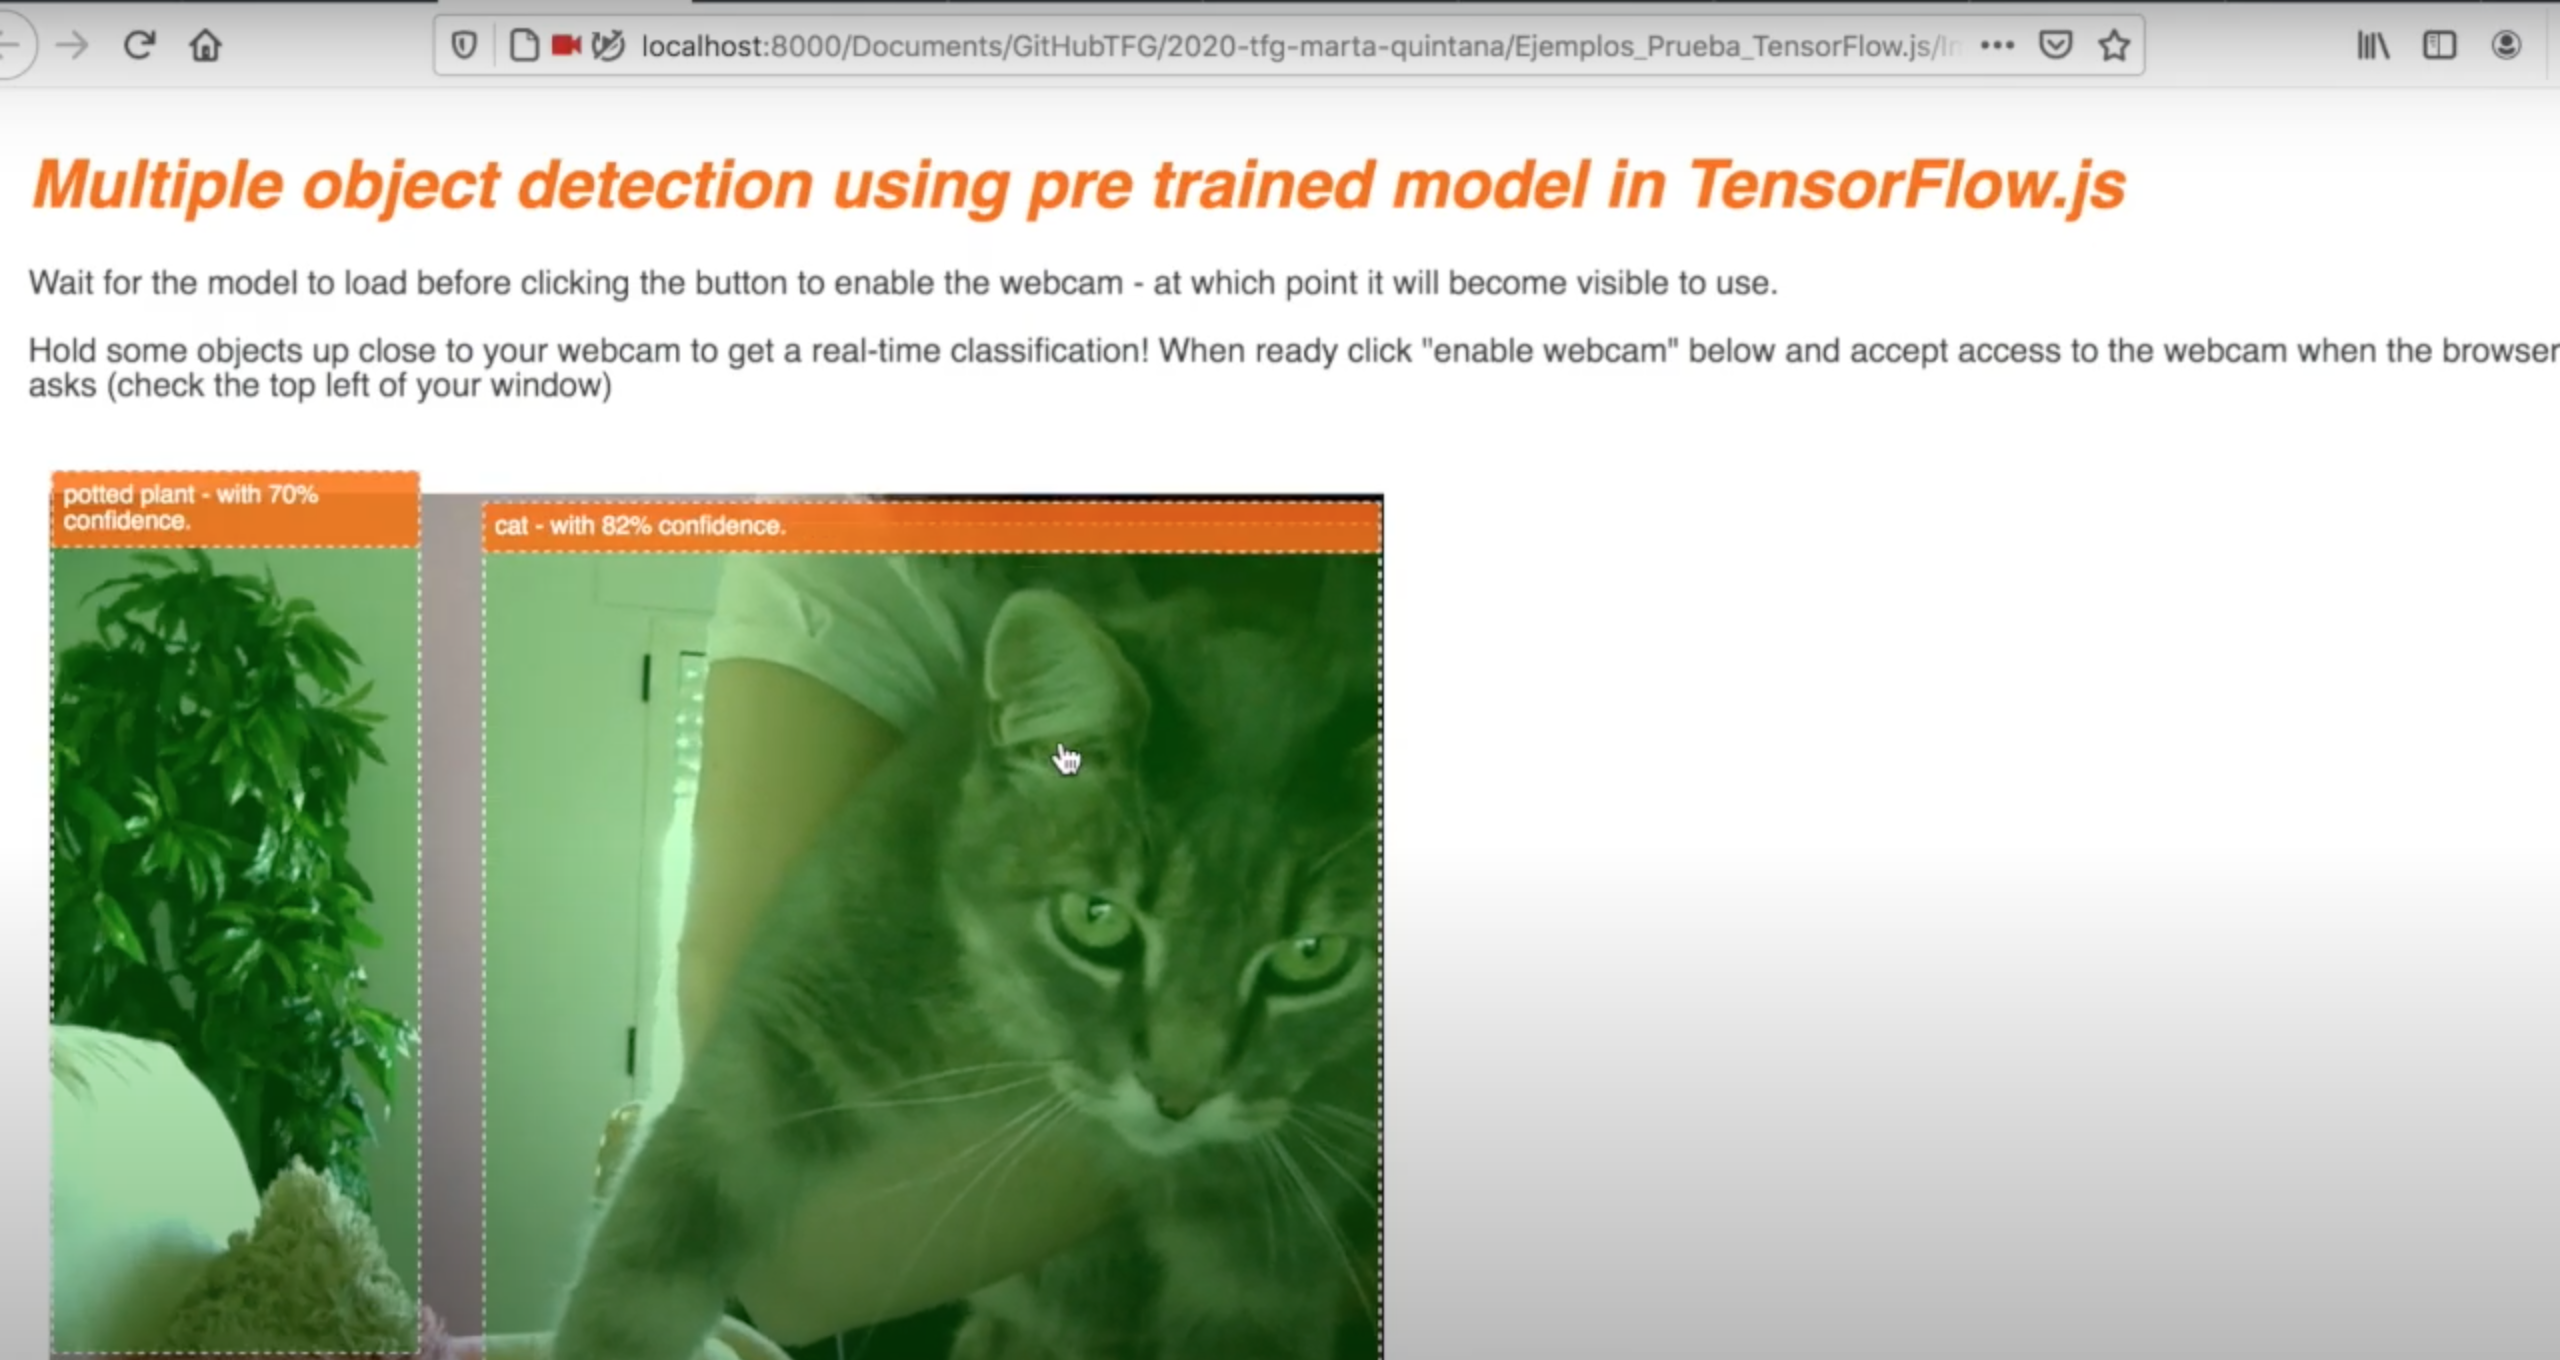
\includegraphics[width=0.8\textwidth, height=0.4\textwidth]{chapters/images/imagerecognition.png}
    \caption{Tensor Flow JS ejemplo detección de objetos. }
    \label{fig:my_label}
\end{figure}

Con Tensor Flow se hicieron dos prototipos uno con un modelo pre-entrenado que reconocía 10 palabras entre ellas go, stop, right, left  y seven que se utilizó para que el robot fuera hacia atrás.
Este modelo al ser pre-entrenado y definido por TensorFlowJS no era muy exacto y el ruido de fondo afectaba demasiado a la hora de detectar cada palabra en nuestro ejercicio. Por ello, el segundo prototipo se hizo con un modelo que se entrenaba con la voz del alumno que usara ese ejercicio.

En este segundo prototipo cada palabra necesitaba grabar sus muestras, al menos unas 100 muestras por palabra, incluidas las muestras de ruido de fondo para que la detección fuera más precisa. Este modelo funcionaba más o menos bien pero no era lo más adecuado para el ejercicio que se había planteado. A pesar de que funcionaba bien se descartó porque era una tarrea muy laboriosa de grabar todas las muestras cada vez que entrabas en el ejercicio. 
En estos videos \footnote{https://www.youtube.com/watch?v=DcwJzCOE4kI}
\footnote{https://www.youtube.com/watch?v=nPeCAb47jiU}** se puede ver  como eran estos modelos y como funcionaban con un drone.
.  **GRABAR VIDEO TELEOP TENSOR FLOW JS CON TODO.

Investigando el mundo de reconocimiento de audio y JavaScript se descubrió la herramienta Teachable Machine, la tecnología  que finalmente se ha usado en este proyecto.

Teachable Machine es una herramienta basada en la Web para crear modelos de aprendizaje automático destaca por modelos de clasificación de imagenes, sonidos y posturas. Teachable Machine internamente usa TensorFlow\.js . 

La creación de un modelo en Teachable Machine tiene 3 fases: recopilación, preparación y exportación del modelo a tu proyecto.

\begin{itemize}
\item \textit{Recopilación}: primero hay que recopilar muestras, para ello fue necesaria la participación de 10 personas diferentes para que el modelo fuera más completo y pudiera reconocer la palabra independientemente de si la voz del usuarios  es más aguda o más grabe.  Se usaron aproximadamente 10 muestras de cada palabra por persona. El modelo cuenta con 105 muestras por cada palabra (10 muestras x 10 personas). Las palabras que queremos reconocer son \textit{go, stop, back, right, left, up, down } y el ruido de fondo. Esto ha supuesto un total de 840 muestras.

Las muestras se grabaron una a una en la página de creación de modelos de Teachable Machine en la Figura 4.2 se puede ver el modelo y las muestras grabadas.


\begin{figure}[H]
 \centering
    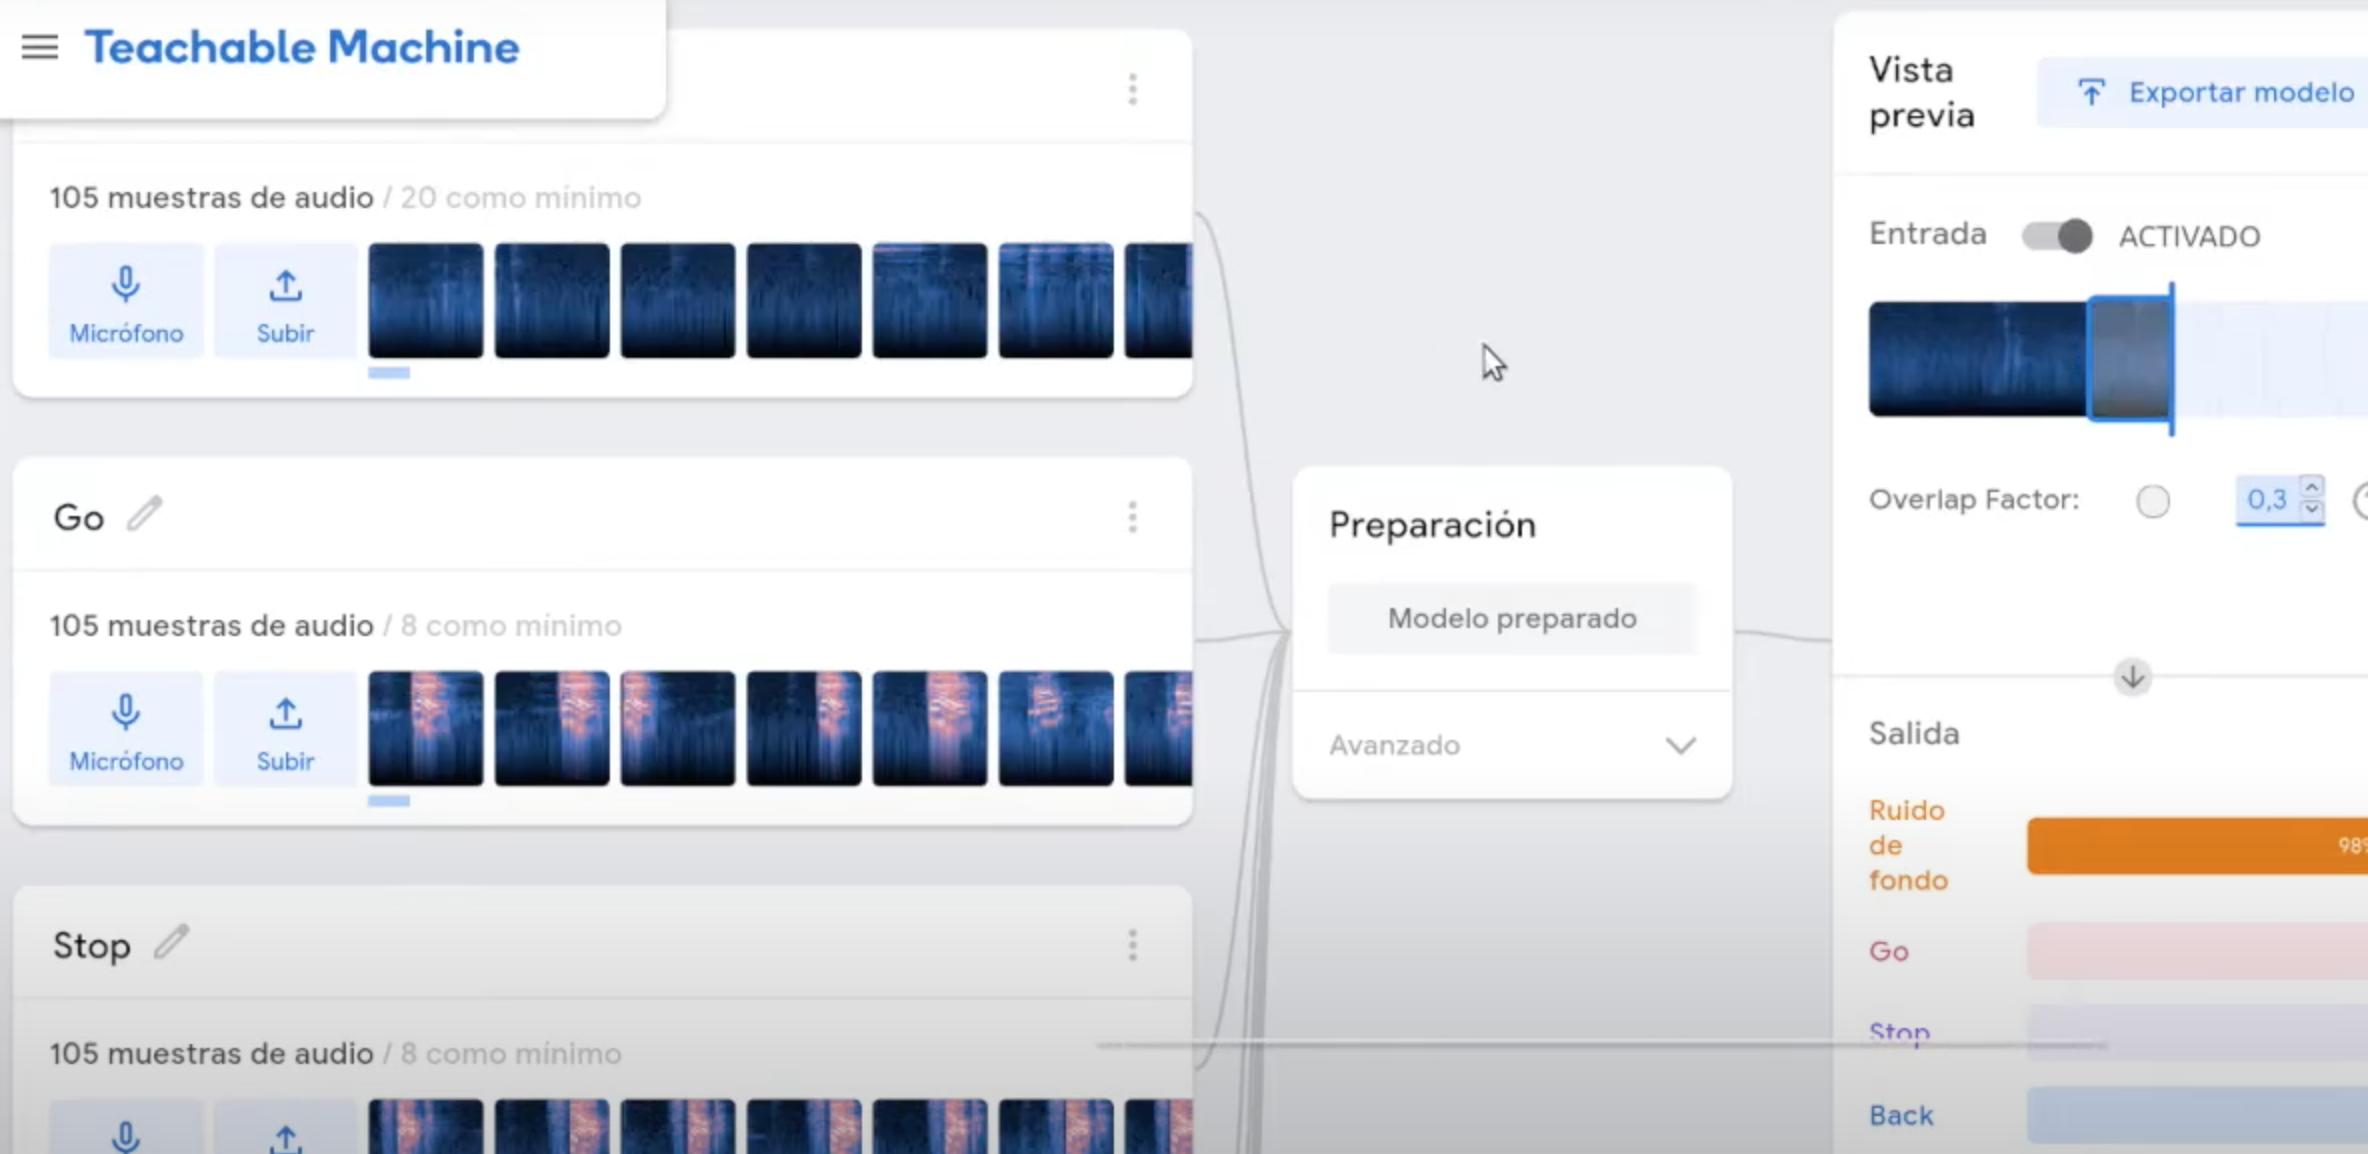
\includegraphics[width=0.8\textwidth, height=0.4\textwidth]{chapters/images/teachablemachine.png}
    \caption{Modelo realizado en Teachable Machine}
\end{figure}
 


\item  \textit{Preparación}

Una vez conseguidas todas las muestras, hay que preparar el modelo. Teachable machine permite cambiar las épocas. Gracias a unas tablas de precisión y pérdidas por época puedes guiarte para  que en función de tus datos puedas ajustar este parámetro, para este proyecto se utilizaron los valores predeterminados que nos proporcionaban  buenos resultados.


\item  \textit{Exportación del modelo a Websim}
Una vez preparado el modelo la página te muestra una vista previa de tu modelo en el que puedes probar y ver el porcentaje de aciertos de cada palabra de tu modelo y con esto decidir si necesitas añadir más muestras o cambiar los parámetros del modelo.  En la Figura 4.3 podemos ver como ya esta listo nuestro modelo y la página nos deja probarlo para hacer los cambios necesarios.

\begin{figure}[H]
 \centering
    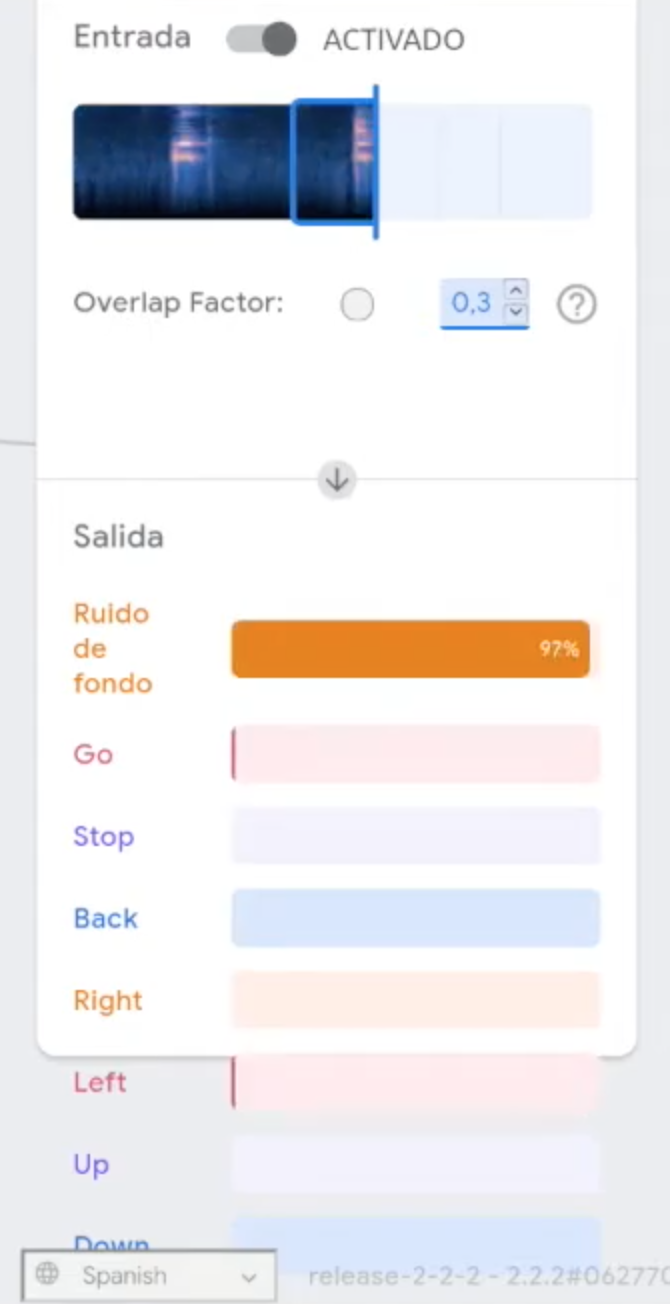
\includegraphics[width=0.4\textwidth, height=0.6\textwidth]{chapters/images/teachablemachine2.png}
    \caption{Vista previa del modelo}
\end{figure}
 

Una vez ajustado y con las 105 muestras por palabra, se exportó el modelo. 
Para exportarlo Teachable Machine lo puede alojar en sus servidores y te proporciona de enlace de forma gratuita o puedes descargarlo, se optó por alojarlo en la nube de Teachable Machine para que no ocupara mucho espacio en Kibotics, ya que la forma de importarlo  a JavaScriot era similar en ambas opciones.
Una vez subido el modelo, Teachable machine te proporciona una URL de la dirección de tu modelo y  te proporciona el código necesario para importarlo a tu proyecto desde JavaScript.
\end{itemize}

Con estos 3 pasos ya tenemos creado nuestro modelo en  Teachable Machine. En el Anexo A se puede ver como implementó una primer prueba de ejemplo sin asignarlo al comportamiento del robot en Websim.

Una vezse comprobó que el modelo funcionaba, se estudió como incorporar el modelo de reconocimiento de audio en Websim, para ello  se creó el siguiente fichero audio\.js que se importa en el html del ejercicio de la siguiente forma:   

\textless script type=``''text/javascript" src=``''js/audio.js" \textgreater

Código de audio.js:

\begin{lstlisting}
document.addEventListener('robot-loaded', (evt)=>{
  localRobot = evt.detail;
  console.log(localRobot);
});
// more documentation available at
// https://github.com/tensorflow/tfjs-models/tree/master/speech-commands

// the link to your model provided by Teachable Machine export panel
const URL = "https://teachablemachine.withgoogle.com/models/P3XdF5r5d/";
var connection = false;
var noise_times = 0;

async function createModel() {
    const checkpointURL = URL + "model.json"; // model topology
    const metadataURL = URL + "metadata.json"; // model metadata

    const recognizer = speechCommands.create(
        "BROWSER_FFT", // fourier transform type, not useful to change
        undefined, // speech commands vocabulary feature, not useful for your models
        checkpointURL,
        metadataURL);

    // check that model and metadata are loaded via HTTPS requests.
    await recognizer.ensureModelLoaded();

    return recognizer;
}

async function analizar(recognizer,classLabels,word) {
//  for (let i = 0; i < classLabels.length; i++) {
  //    labelContainer.appendChild(document.createElement("div"));
  //}

  // listen() takes two arguments:
  // 1. A callback function that is invoked anytime a word is recognized.
  // 2. A configuration object with adjustable fields
  recognizer.listen(result => {
      console.log(noise_times)
      const scores = result.scores; // probability of prediction for each class
      var word_index = 0;

      // render the probability scores per class
      for (let i = 0; i < classLabels.length; i++) {
          const classPrediction = classLabels[i] + ": " + result.scores[i].toFixed(2);
          //labelContainer.childNodes[i].innerHTML = classPrediction;
          //The most probable word
          if (result.scores[i].toFixed(2) >= result.scores[word_index].toFixed(2)) {
             word_index = i;
          }
      }
      var prediction = classLabels[word_index];
      word.innerHTML = "The most probable word: " + prediction;
      if (String(prediction) == "_background_noise_"){
        noise_times = noise_times + 1;
      }else{
        noise_times = 0;
      }
      if (connection){
        if (String(prediction) == "Go") {
          localRobot.setV(0.9);
          //que se mueva el robot
        }else if (String(prediction) == "Stop") {
           localRobot.setV(0);
           localRobot.setW(0);
           localRobot.setL(0);
          //que se pare
        }else if (String(prediction) == "Back"){
           localRobot.setV(-0.9);
        }else if (String(prediction) == "Right"){
            localRobot.setW(-0.005);

        }else if (String(prediction) == "Left"){
            localRobot.setW(0.005);

        }else if (String(prediction) == "Up"){
            localRobot.setL(0.25);

        }else if (String(prediction) == "Down"){
            noise_times = 0;
            console.log(localRobot.velocity);
            if (localRobot.velocity.y = 0.25) {
              localRobot.setL(-0.25);
            }
        }
        //For stop going down or going up, turn left or turn right say the word : STOP

      }
      //console.log(prediction);
  }, {
      includeSpectrogram: true, // in case listen should return result.spectrogram
      probabilityThreshold: 0.75,
      invokeCallbackOnNoiseAndUnknown: true,
      overlapFactor: 0.50 // probably want between 0.5 and 0.75. More info in README
  });

  // Stop the recognition in 10 seconds.
  setTimeout(() => {recognizer.stopListening(); }, 10000);

}

async function listen() {
        document.getElementById("listen_again").style.visibility = 'hidden';
        //--------TEACHABLE MACHINE--------------
        const recognizer = await createModel();
        const classLabels = recognizer.wordLabels(); // get class labels
        //const labelContainer = document.getElementById("label-container");
        const word = document.getElementById("prediction");
      //  for (let i = 0; i < classLabels.length; i++) {
        //    labasync function listen() {elContainer.appendChild(document.createElement("div"));
        //}

       var id = setInterval(() => {if(noise_times <= 10){analizar(recognizer,classLabels,word)}else{
          setTimeout(() => {console.log("Se ha parado de analizar")
            word.innerHTML = "The most probable word: " ;
            clearInterval(id);
            document.getElementById("listen_again").style.visibility = 'visible';
            //Robot Control opcional
            //localRobot.setV(0);
            //localRobot.setW(0);
            //localRobot.setL(0);
          }, 10000);
        }}, 10150);

}

async function Back\_To\_Listen(){
   document.getElementById("prediction").innerHTML= 'The most probable word: <br> <img src="https://wbl.telcel\-id.com:8443/images/Load\_Icon.gif" alt="Loading the model">'
   noise\_times = 0;
   listen();
}



async function Connect\_To\_Robot() {
    if (connection){connection= false;
      document.getElementById(``connection").style.backgroundColor= "red";
      console.log( "Desconectado");
    }else{
        connection = true;
        listen();
        console.log( "CONECTADO AL ROBOT");
        document.getElementById(``connection").style.backgroundColor= "green";
    }
}
\end{lstlisting}

A continuación se explica como funciona este programa.

Cuando se pulsa al boton Conect\_To\_Robot se llama a la función del mismo nombre que internamente ejecuta  la funcion listen() que es la que inicializa el reconocimiento y analiza el audio cada 10 segundos.
Este botón Conect\_To\_Robot  se pone en verde cuando esta analizando y en rojo cuando está desconectado, esto quiere decir que el robot no reconoce ninguna palabra mientras el botón esté de ese color.
La función listen() inicializa el modelo y crea las etiquetas que necesita, una vez se crea el modelo se ha creado un setTimeout para esperar 10 segundos hasta que cargue el modelo. Cuando este carga, se establece un setInterval para que cada 10 segundos se ejecute la función analizar que devuelve la palabra estimada.

La función analizar es la que invoca al analizador o \textit{recognizer}, en él se predice la palabra que cree que es más probable que haya dicho el usuario.  \textit{Prediction} es esa palabra que tiene  la probabilidad más alta.

Una vez tenemos la \textit{prediction} se compara esta palabra con la 8 palabras que hemos entrenado el modelo \textit{go, stop, back, right, left, up, down y \_background\_noise\_}

Gracias al evento 'robot-loaded' cuando el robot está cargado en el escenario,  obtenemos el objeto localRobot, que en nuestro ejercicio es el dron. En Kibotics poseen una API con funciones para controlar el movimiento del robot.  Cuando se predice una de las 8 palabras en los condicionales \textit{if(){} else if() {}}se llama a una de las distintas funciones de velocidad que se pueden fijar: localRobot.setV(), para asignar la velocidad lineal se utiliza para ir hacia delante ``go'', ir hacia atrás ``back '' y parar ``stop'',  localRobot.setW() para la velocidad angular, se usa para girar a la derecha``right'' y a la izquierda`left`'' y  localRobot.setL() para asignar la velocidad que va a subir ``up'' y bajar ``down'' el drone. Si se predice que es ruido de fondo no afecta en el comportamiento del drone.

La implementación del ejercicio con Teachable Machine  aporta sencillez y más precisión que los modelos mencionados anteriormente.
Una vez realizado el ejercicio se optimizó para que el navegador del usuario no estuviera todo el tiempo analizando el  audio si no tenemos nada que decirle al dron y aprovechar  los recursos del ordenador usuario.

La optimización se realizó añadiendo un contador de las veces que se predice ruido de fondo \textit{noise\_times}. Se estableció un máximo de 10 las veces seguidas que la predicción es \textit{\_background\_noise\_}. Como se analiza el audio cada 10 segundos esto quiere decir que si han pasado 100 segundos y siempre ha detectado ruido de fondo, la función analizar para de ejecutarse y no se predice ninguna palabra. Cuando ocurre esto se muestra en el navegador un nuevo botón \textit{Continue analizing} que  si lo pulsas desaparece y se vuelve a reiniciar el procesamiento de audio.

**FOTOS

Finalmente al fichero de configuración del drone que se usaba anteriormente se añadió una portería de rugby con Blender y una pared para añadir obstáculos a los escenarios.

\subsection{Solución de referencia}
Este ejercicio no tiene una solución de referencia como los siguientes que vamos a ver a lo largo del trabajo. Es un juego en el que tienes que dirigir al dron con tu voz para cruzar por la portería de rugby o pasar de un lado al otro de la pared sin chocarte con ellas.

**FOTOS Elemplo


\section{Banda Sonora}

Para añadir banda sonora a los ejercicios existentes en Kibotics, se estudió como inserar audio desde html5 e implementarlo con JavaScript en Websim.

El elemento HTML \textless audio \textgreater  se usa para reproducir un fichero de audio en una página web.
Los atributos que destacan de este elemento son \textit{controls, source, loop y autoplay }.
El atributo \textit{controls} proporciona controles como reproducir, parar y subir o bajar el volumen.
 \textit{Source} permite especificar la fuente de audio, en este caso un fichero en formato mp3, ogg o wav. \textit{Loop} permite volver a reproducir el audio cuando este se acabe, el audio estará en bucle y \textit{autoplay} se utiliza para que una vez se cargue el fichero de audio, este empiece a reproducirse.

Para implementar esta mejora a Kibotics en la carpeta assets de Websim se añadió una nueva carpeta llamada ``soundtracks'' con temas musicales para poner en los ejercicios. Las canciones usadas son de Patrick De Artega Royalty Free Music  \footnote{ https://patrickdearteaga.com Credits to Patrick De Artega Royalty Free Music 2020}
y los temas que se han añadido son:
\begin{itemize}
	\item Chiptronical 
	\item Common Fight 
	\item Goliath's Foe 
	\item Resilience 
	\item Spring Village 
	\item TheTrueStory of Beelzebub 
	\item Vals de su jardín
\end{itemize}

La banda sonora de cada ejercicio se define en su fichero de configuración. En ese fichero se ha creado un objeto con una  la etiqueta  ``soundtrack'', el identificador ``audio'' y la dirección del fichero fuente del audio que se quiere asignar como banda sonora como se muestra en el siguiente código:

\begin{lstlisting}
 	{"tag":"soundtrack",
        "attr": {
            "id":"audio",
            "src": "../assets/soundtracks/Spring\_Village.ogg"
          }
        },
   \end{lstlisting}

Websim tiene un analizador de ficheros json llamado config\_parser.js, en ese fichero se analiza el fichero de configuración con el objeto que hemos mencionado anteriormente y traducirlo a A-Frame.

Cuando Websim lee el código del fichero de configuración (formato JSON) se llama a parseSoundtrack() que recibe los objetos de la escena para analizar si hay banda sonora o no en el ejercicio.

\begin{lstlisting}
 	await parseSoundtrack(sceneObjects);
\end{lstlisting}

En el siguiente código se muestra como se analizan todos los objetos de la escena y si alguno tiene la etiqueta ``soundtrack'', la variable soundtrack  que por defecto siempre es false, pasa a ser true y se asigna a la variable audio el atributo  'src' del objeto, en este caso "../assets/soundtracks/Spring\_Village.ogg".  
Si soundtrack es true, se crea un objeto Audio() de HTML5 desde JavaScript; y se le asigna el src del audio configurado y se empieza a reproducir. Como reproducir.loop es true, el audio estará en bucle todo el tiempo.

\begin{lstlisting}
export function parseSoundtrack(sceneObjects){
  var soundtrack = false;
  for (var i = 0; i <sceneObjects.length;i++){
   if (sceneObjects[i]['tag']== 'soundtrack'){
     soundtrack = true;
     var audio=sceneObjects[i]['attr']['src'];
    }
  }
  if (soundtrack) {
    var reproducir = new Audio();
        reproducir.src= audio
        reproducir.loop= true;
        reproducir.play();
  }
  return;
}
\end{lstlisting}

En este video \footnote{https://www.youtube.com/watch?v=c\_\_BayBCSX4} se puede escuchar la banda sonora que se ha asignado en un ejercicio de ejemplo.

\subsection{Efecto de sonido por colisión }

Los efectos de sonido son muy importantes en los juegos, es por ello que se pensó mejorar la experiencia del usuario añadiendo el efecto de sonido de colisión. 

Se implementó con el evento 'collide' de A-Frame y se asigna y reproduce un audio cuando se choca y todas las velocidades V, W y L del robot se ponen a 0.  En este caso la reproducción del audio se hace una vez por choque como pasaría en la realidad.

\begin{lstlisting}
  document.addEventListener('collide', function (e) {
      console.log('Robot has collided!');
      var reproducir = new Audio();
      reproducir.src= 'http://sonidosmp3gratis.com/sounds/000215403\_prev.mp3';   //collision sound
      reproducir.play();
      localRobot.setV(0);
      localRobot.setW(0);
      localRobot.setL(0);
	});
	
\end{lstlisting}

Esta función sirve para todos los ejercicios de la plataforma con o sin  bandas sonoras y para el teleoperador acústico.